%% \typeout{IJCAI--22 Instructions for Authors}

% These are the instructions for authors for IJCAI-22.

\documentclass{article}
\pdfpagewidth=8.5in
\pdfpageheight=11in
% The file ijcai22.sty is NOT the same as previous years'
\usepackage{ijcai22}

% Use the postscript times font!
\usepackage{times}
\usepackage{soul}
\usepackage{url}
\usepackage[hidelinks]{hyperref}
\usepackage[utf8]{inputenc}
\usepackage[small]{caption}
\usepackage{graphicx}
\usepackage{amsmath}
\usepackage{amsthm}
\usepackage{booktabs}
\usepackage{algorithm}
\usepackage{algorithmic}
\usepackage{multirow}
\urlstyle{same}

% the following package is optional:
%\usepackage{latexsym}

% See https://www.overleaf.com/learn/latex/theorems_and_proofs
% for a nice explanation of how to define new theorems, but keep
% in mind that the amsthm package is already included in this
% template and that you must *not* alter the styling.
% \newtheorem{example}{Example}
% \newtheorem{theorem}{Theorem}

% Following comment is from ijcai97-submit.tex:
% The preparation of these files was supported by Schlumberger Palo Alto
% Research, AT\&T Bell Laboratories, and Morgan Kaufmann Publishers.
% Shirley Jowell, of Morgan Kaufmann Publishers, and Peter F.
% Patel-Schneider, of AT\&T Bell Laboratories collaborated on their
% preparation.

% These instructions can be modified and used in other conferences as long
% as credit to the authors and supporting agencies is retained, this notice
% is not changed, and further modification or reuse is not restricted.
% Neither Shirley Jowell nor Peter F. Patel-Schneider can be listed as
% contacts for providing assistance without their prior permission.

% To use for other conferences, change references to files and the
% conference appropriate and use other authors, contacts, publishers, and
% organizations.
% Also change the deadline and address for returning papers and the length and
% page charge instructions.
% Put where the files are available in the appropriate places.

% PDF Info Is REQUIRED.
% Please **do not** include Title and Author information
\pdfinfo{
  /TemplateVersion (IJCAI.2022.0)
}

\title{IJCAI--22 Formatting Instructions}

% Single author syntax
%% \author{
%%     Author Name
%%     \affiliations
%%     Affiliation
%%     \emails
%%     pcchair@ijcai-22.org
%% }

% Multiple author syntax (remove the single-author syntax above and the \iffalse ... \fi here)

\author{
  Arumoy Shome$^1$
  \and
  Lu{\'\i}s Cruz$^1$\And
  Arie van Deursen$^{1}$
  \affiliations
  $^1$Delft University of Technology\\
  \emails
  \{a.shome, l.cruz, arie.vandeursen\}@tudelft.nl
}


\begin{document}

\maketitle

\begin{abstract}
  %% TODO
\end{abstract}

\section{Introduction}\label{sec:intro}
%% TODO

%% fairness & accountability are now part of AI legislation; we need
%% to test for to ensure modern AI systems are not driven by bias;
%% however testing such complex systems can not only be challenging
%% but also incures costs in terms of compute & time; we want to catch
%% such problems as early as possible...

%% present a general motivation of the problem space & the problem we
%% are trying to solve

%% present research questions that we want to answer along with brief
%% preview of results

%% can we rely (with statistical guarantee) that the data fairness
%% metrics identifies fairness issues in the model as well? to what
%% extend does this relationship hold?

%% RQ1: is there a relationship between DFM and MFM?
%% RQ1.2: does this relationship hold as the underlying distribution
%% of the data changes?
%% RQ2: does this relationship hold as the underlying features in the
%% dataset change?

\section{Background \& Related Work}\label{sec:related}

%% summarise the current work on fairness testing; touch upon this
%% aspect from a SE perspective; the fairness metrics we have (and why
%% we use specific ones);

%% TODO (brief) review on test prioritisation/minimisation from SE &
%% ML perspective

%% TODO brief overview of group fairness & the metrics we are using in
%% this study along with the datasets.

\begin{table}
  \centering
  \caption{Datasets used in the study}
  \begin{tabular}{p{0.3\linewidth} p{0.1\linewidth} p{0.1\linewidth} r}
    \toprule
    \textbf{Name} & \textbf{Prot.} & \textbf{Abbr.} &
    \textbf{Total Examples}\\
    \midrule
    \multirow{2}{*}{German Credit \cite{CITEME}} & age & GA &
    1000\\
      & sex & GS & 1000\\
    \multirow{2}{*}{Compas Score \cite{CITEME}} & race & CR &
    6167\\
      & sex & CS & 6167\\
    Medical Survey 2021 \cite{CITEME} & race & MR & 15675\\
    Bank Marketing \cite{CITEME} & age & BA & 30488\\
    \multirow{2}{*}{Adult Income \cite{CITEME}} & race & AR & 45222\\
      & sex & AS & 45222\\
    \bottomrule
  \end{tabular}
  \label{tab:datasets}
\end{table}
%% TODO brief commentary on tab:datasets, the ones we use (and why),
%% the range of examples; short comment on pre-existing bias in the
%% dataset.

%% list the fairness metrics we use in our analysis & why


\begin{equation}
  DI_{data} = \frac{P(Y=1|D=0)}{P(Y=1|D=1)}
  \label{eq:di-data}
\end{equation}

\begin{equation}
  DI_{model} = \frac{P(\hat{Y}=1|D=0)}{P(\hat{Y}=1|D=1)}
  \label{eq:di-model}
\end{equation}

\begin{equation}
  SPD_{data} = P(Y=1|D=0)-P(Y=1|D=1)
  \label{eq:spd-data}
\end{equation}

\begin{equation}
  DI_{model} = P(\hat{Y}=1|D=0)-P(\hat{Y}=1|D=1)
  \label{eq:spd-model}
\end{equation}

%% list the ML models we use in our analysis and why (because we want
%% to generalise over multiple datasets)

\section{Methodology}\label{sec:method}
%% TODO should we include numbers conditioned on
%% privileged/unprivileged?

%% - we use 5 popular datasets from the fairness literature
%% - we use 4 popular ML models used in prior fairness testing
%% literature
%% - we use 2 popular group fairness metrics used in the fairness
%% literature
%% - we calculate fairness metrics first on the data (DFM) and next on
%% the predictions of the model on the test set (MFM) and analyse the
%% results
%% - we normalise all results following the procedure used by
%% zhang2021ignorance 
%% - we use correlation & linear regression to analyse the
%% relationship between DFM & MFM; we observe that they are related to
%% one another; DFM can indicate fairness issues in the model with
%% statistical significance

%% spearman correlation is less sensitive to outliers and does not
%% assume normality which is why we use it in our analysis

%% verify the assumptions of linear regressions are validated & met in
%% our analysis; we check the coefficient of determination (R^2) which
%% is a general measure for goodness of fit; value close to 1
%% indicates variability in y is explained by the regression model
%% (ie. by x); we also check the plot of residuals against fitted
%% values: if most data is centered around 0 and evenly spread then it
%% indicates a linear relationship with constant variability

%% outline the data collection setup; break this down by the
%% experiments (we have two); explain the slicing mechanism in each
%% experiment, how & why we are shuffling the example & feature orders

%% TODO definitely need to diagram; hard to explain experimental
%% design using only words

%% we only consider one protected attribute at a time; for feature
%% sets experiment, we consider a minimum of 3 features (in addition
%% to the protected attribute & target features)

\begin{figure*}
  \centering
  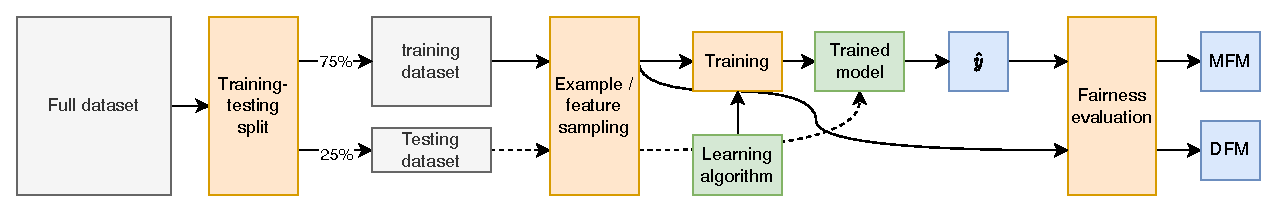
\includegraphics[width=0.95\linewidth]{method.pdf}
  \caption{Methodology for data collection and analysis}
  \label{fig:method}
\end{figure*}

Figure \ref{fig:method} presents the experimental design for the
study. For each dataset, protected attribute and model tuple, we use a
75-25 split with shuffling to create the training and test sets. For
the experiment

%% we quantity the bias in the underlying distribution of the training
%% data by evaluating the fairness metrics using only the training
%% data; we quantify the bias in the model after training by
%% calculating fairness metrics using the predictions of the model on
%% the test set

We calculate the DFMs on the training set and the MFMs on the
predictions of the model on the test set. Next we analyse the DFM and
MFM by observing the correlation between them and by fitting a linear
regression model. We repeat this procedure 50 times and use
statistical hypothesis testing to validate that our results are
statistically significant.

We extend the above experiment further in two ways (by adopting the
experimental design from \cite{zhang2021ignorance}). First, we
experiment with different number of training examples and second with
different number of features in the training set. For both examples,
we shuffle the order of the examples in the training and test sets. For
the feature sets experiment, we additionally shuffle the order of the
features.

For the training sets experiment, we create different sub-subsets of
the training subset from 10\% to 100\%. For the feature sets
experiment, we consider a minimum of 3 features (in addition to the
protected attribute and the target feature) to all features.

% TODO mention that we check the statistical significance of the
% correlation & linear regression analysis by observing the p values
% at 3 alpha levels: 0.01, 0.05 & 0.1

\section{Results}\label{sec:results}
%% introduce the experiments and results briefly; other general info
%% that is used across all experiments can be reported here;

\subsection{Full Training Set}\label{sec:results-full-data}

\begin{figure}
  \centering
  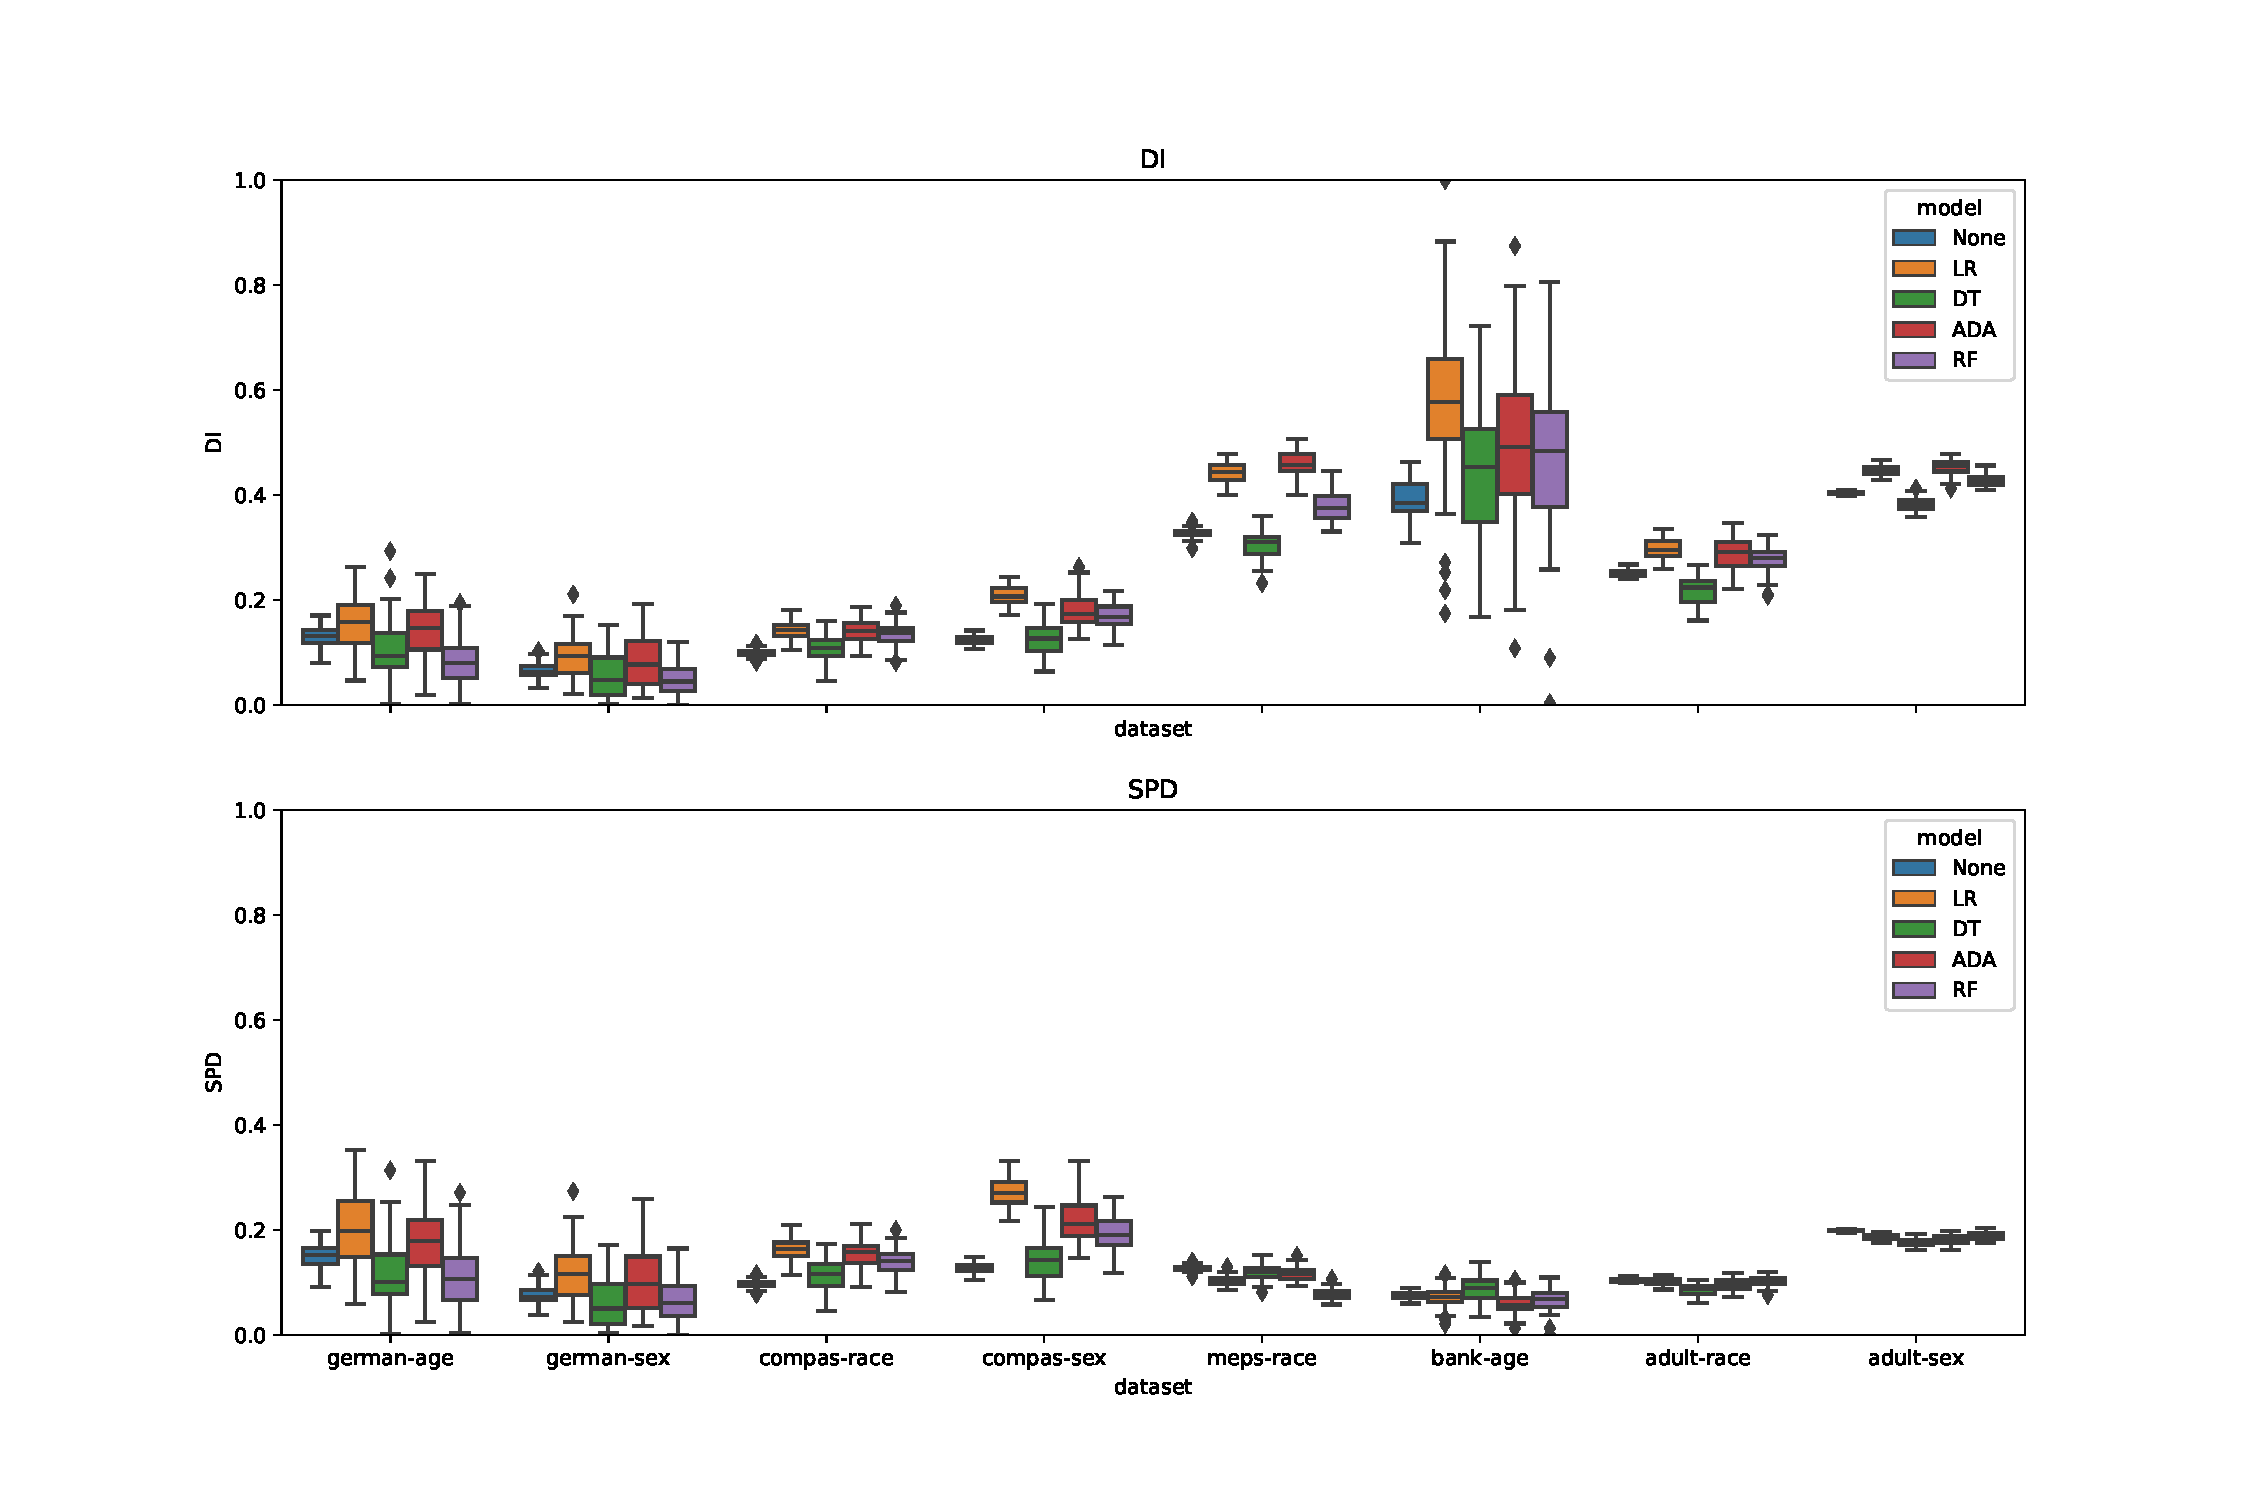
\includegraphics[width=0.95\linewidth]{boxplot--dataset--di-spd--exp-full.pdf}
  \caption{Distribution of DFM and MFM across datasets}
  \label{fig:boxplot--dataset--di-spd--exp-full}
\end{figure}

In this section we analyse the relationship between the DFM and MFM
when the full training dataset is used to train the models.
Figure \ref{fig:boxplot--dataset--di-spd--exp-full} presents the
distribution of the fairness metrics across the datasets. We observe
that DFM and MFM convey similar information in all cases. The
variability of the DFM is lesser compared to the MFM. This is because
in addition to the randomness from the data shuffling in the training
set, the models are assigned random initial states in every iteration.
Finally in several cases the tree based classifiers (DT and RF) make
fairer decisions compared to the other classifiers, sometimes even
better than the baseline provided by the DFM.

%% TODO not sure if we should include the comment on the tree based
%% models; we don't touch upon this in the subsequent sections of the
%% report

% We observe an anomaly in the distribution of the fairness metrics in
% the bank-age dataset. This is due the persence of severe bias in the
% underlying dataset. The bank-age dataset contains 3586 examples of
% privileged positive while only 273 examples of unprivileged
% positive which may explain the higher degree of variability in the
% fairness metrics. We do not see this variability in the SPD metric,
% however we cannot draw a direct comparision between DI and SPD since
% they have different mathematical formulae (former is a division
% while the later is a subtraction).

Figure \ref{fig:heatmap--corr--full-data} shows the correlation between
the DFM and the MFM across all models and datasets. The significance
of the correlation is indicated by the degree of stars where higher
number of stars indicate lower values of $\alpha$. We test the
significance of the correlation at 3 levels of $\alpha$ namely $0.01$,
$0.05$ and $0.1$. A higher number of stars indicate that the
correlation is statistically significant, and not caused by chance.

We primarily observe darker colors in the heatmap indicating that
there is no correlation between the DFM and MFM in most of the cases.
The distribution of the training dataset changes every iteration since
we shuffle the order of the examples prior to creating the training
and testing sets. However this is not enough to produce a significant
quantity of change and thus consequently no correlation amongst the
DFM and MFM.

%% This is also why we only observe statistically significant correlation
%% in only 14 of the 64 cases.

%% lack of correlation may arise from lack of significant bias in the
%% dataset; thus the DFM and MFM are just random and will never be
%% related; see german-sex for example

\begin{figure}
  \centering
  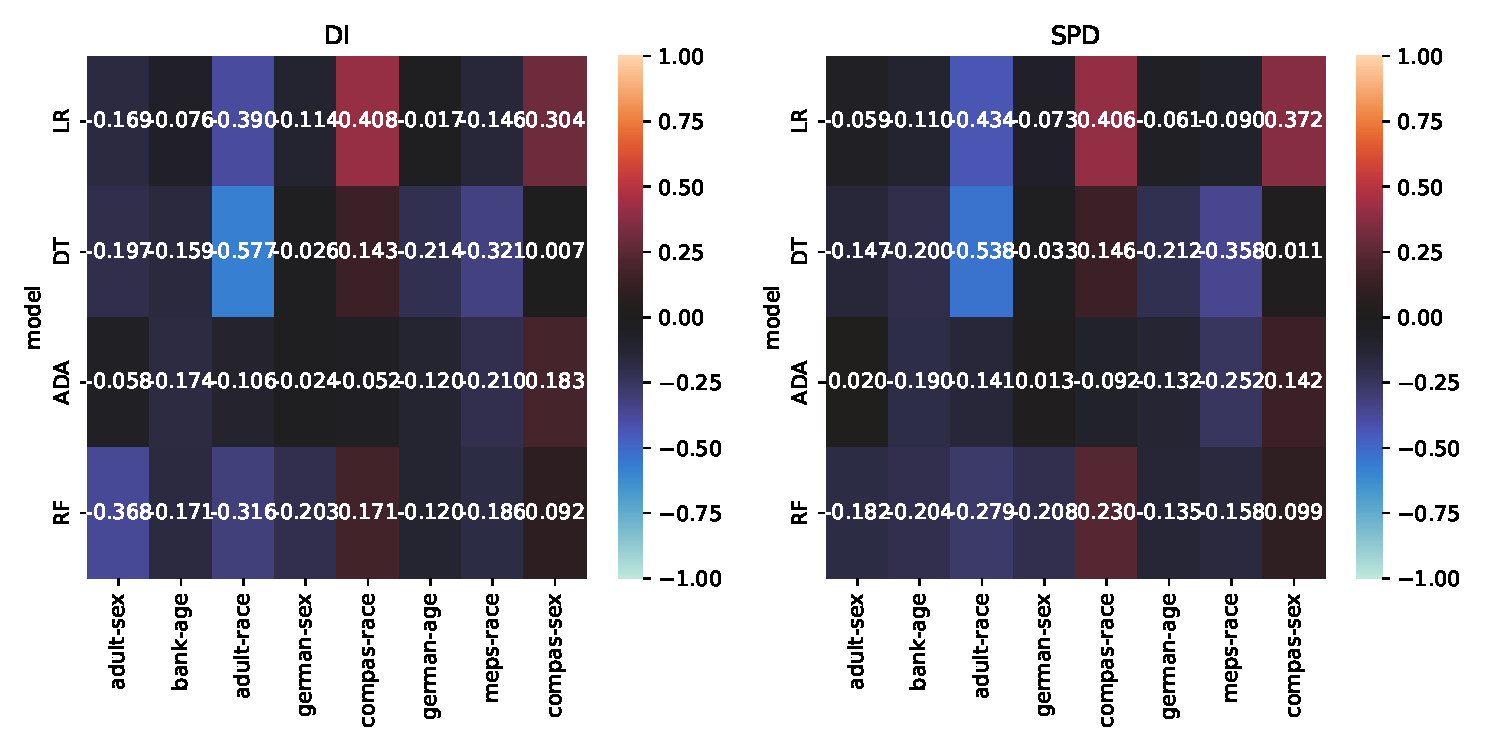
\includegraphics[width=0.95\linewidth]{heatmap--corr--full-data.pdf}
  \caption{Correlation between DFM and MFM}
  \label{fig:heatmap--corr--full-data}
\end{figure}

\subsection{Smaller Training Sets}\label{sec:results-smaller-data}

% %% correlation will depend on the data quantity, quality and model
% %% complexity
% %% we have to check if we have enough data
% %% we have to check if we have bias in the data
% %% both of these are influenced/get influenced by the model we use

As seen in Section \ref{sec:results-full-data}, there is no
significant linear relationship between DFM and MFM due to the lack of
significant change in the distribution of the training dataset across
the 50 iterations. To analyse the relationship between the DFM and MFM
across various data distribution, we modify our experimental design by
calculating the DFM and MFM across varying training size. The data
distribution in smaller training samples will change more frequently
in the 50 iterations at the loss of data quality. To identify a sample
size that captures a variety of data distribution changes while also
being a realistic training dataset, we analyse the \emph{accuracy} and
\emph{f1 score} of the models across the training sample sizes. Next
we conduct \emph{student t-test} to identify the smallest sample size
where the performance of the models is similar to that obtained when
trained using the full training set.

\begin{figure}
  \centering
  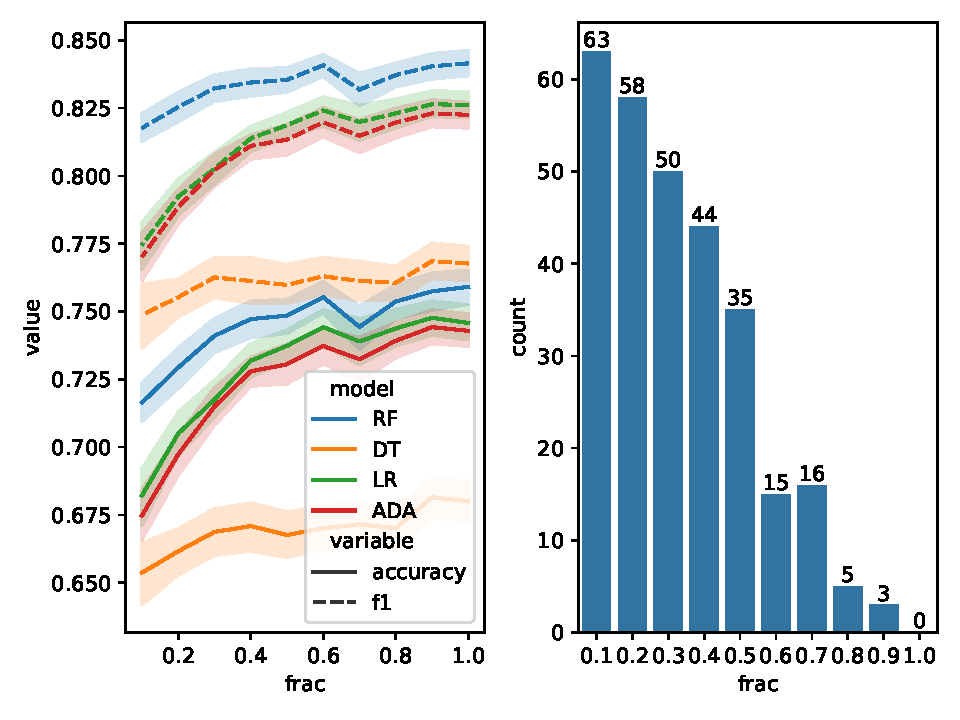
\includegraphics[width=0.95\linewidth]{training-set-frac-threshold.pdf}
  \caption{\emph{\textbf{(left)}} Accuracy and f1 across various
    training sample size in german-age \emph{\textbf{(right)}} Number
    of cases with significant change in accuracy and f1}
  \label{fig:training-set-frac-threshold}
\end{figure}

The right plot in Figure \ref{fig:training-set-frac-threshold} shows
the number of cases where there was a significant difference between
the two populations. We note that there is a significant difference in
the performance of the models in majority of the cases when the
training size is reduced to 50\% while it remains consistent when
using a training size of 60\% and higher. This is also corroborated by
the left plot in Figure \ref{fig:training-set-frac-threshold} which
shows the accuracy and f1 of all models across various training sample
sizes in the german-age dataset. We observe that the performance
metrics are stable until 60\% of the training set is used after which
they drop significantly. Thus for majority of the cases, a training
sample of 60\% allows us to train models with acceptable performance,
while also capturing a wide variety of fairness issues in the
underlying training data within the 50 iterations.

\begin{figure}
  \centering
  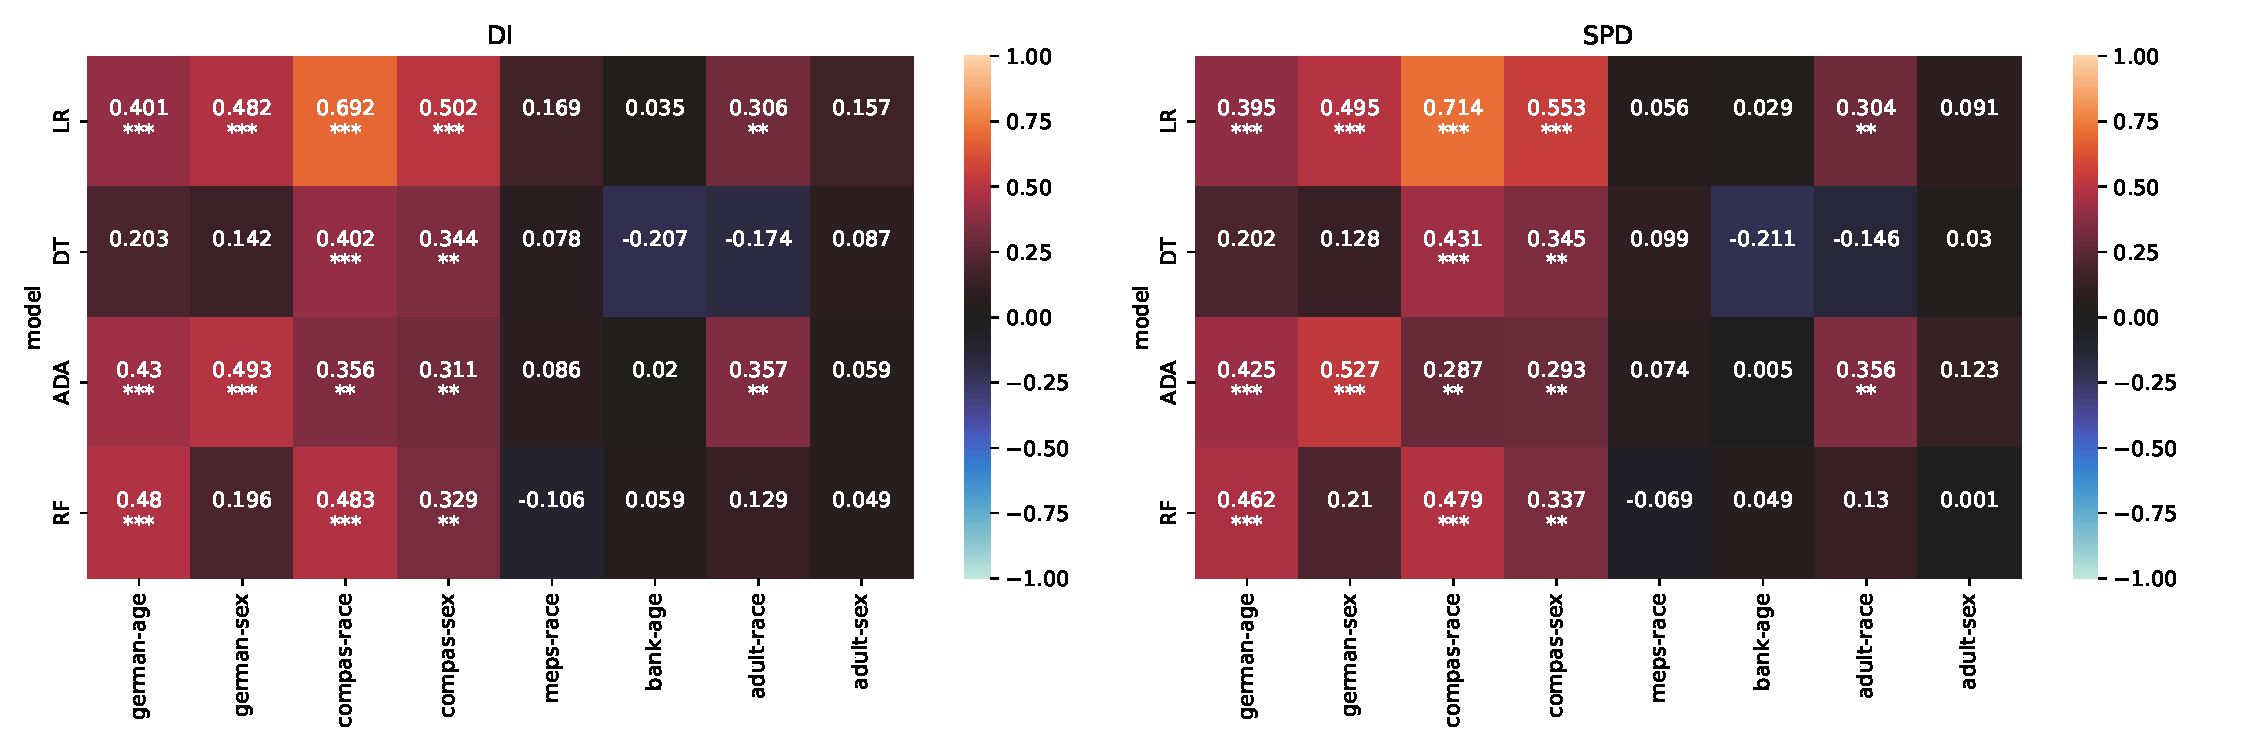
\includegraphics[width=0.95\linewidth]{heatmap--corr--training-sets-frac.pdf}
  \caption{Correlation between DFM and MFM across all models and
    datasets using 60\% training data}
  \label{fig:heatmap--corr--training-sets-frac}
\end{figure}

Figure \ref{fig:heatmap--corr--training-sets-frac} shows the
correlation between the DFM and MFM across all models and datasets
when trained using 60\% of the original training set. In contrast to
Figure \ref{fig:heatmap--corr--full-data}, we primarily observe warmer
colors indicating a positive correlation between the DFM and MFM. This
indicates that the DFM and the MFM convey the same information as the
distribution of the underlying training dataset changes.

\subsection{Correlation across training sample sizes}\label{sec:results-training-sets}

\begin{figure}
  \centering
  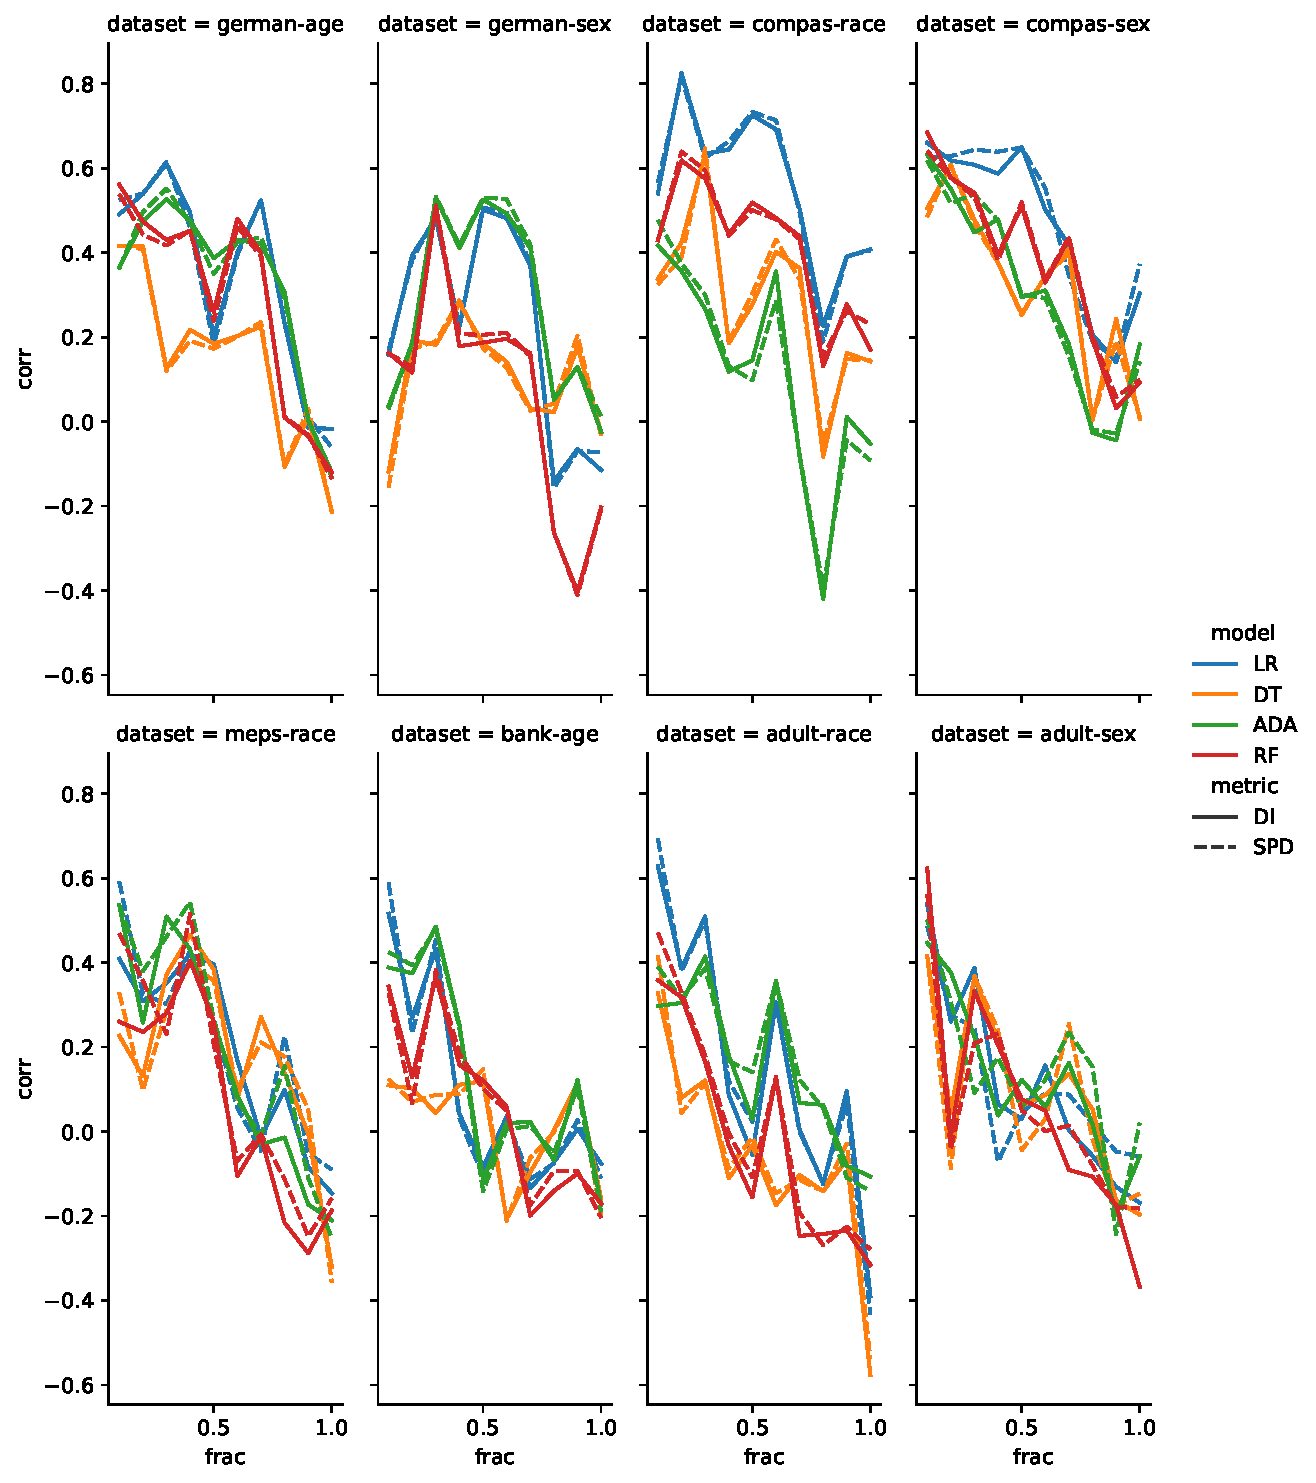
\includegraphics[width=0.95\linewidth]{lineplot--frac--corr.pdf}
  \caption{Distribution of correlation between DFM and MFM across
    various training samples in adult-sex}
  \label{fig:lineplot--frac--corr}
\end{figure}

In Figure \ref{fig:heatmap--corr--full-data} we observe that the
smaller datasets typically have no correlation between DFM and MFM
while the larger datasets typically show a negative correlation. When
we reduce the training sample size to 60\%, the correlation in the
smaller datasets become more positive while the larger datasets
typically do not show any correlation as seen in Figure
 \ref{fig:heatmap--corr--training-sets-frac}. Based on these
observations, we hypothesise that the quantity of training data
influences the fairness in the model. Our hypothesis is corrborated by
Figure \ref{fig:lineplot--frac--corr} which shows the distribution of
the correlation between DFM and MFM across the training samples sizes
in all datasets and models. The overwhelming majority show that the
correlation between the DFM and MFM decreases as we increase the
training size.

% %% don't forget model complexity!

% This indicates that the models are able to make fairer predictions
% with more training data.

%% correlation analysis shows us a general trend; correlation analysis
%% within a specific frac tells us that there is a relationship
%% between DFM and MFM across the iterations; ie. even with the
%% randomness, we see a relationship
%% DFM can be an early indicator for the requirement of more training
%% data although we need to test the model as well (from
%% zhang2021ignorance); more data is wasted if we do not fix the
%% underlying imbalance in the datasets; we can use DFM to test our
%% new samples

%% obv: given enough data, the correlation becomes negative meaning
%% the models are "learning" and making fairer predictions, we know
%% this because DFM will not reduce (it can only go up) since the
%% underlying datasets are biased; thus more data => more unfairness
%% in data => higher DFM

%% move next to correlation across all fracs: now we are analysing the
%% global view: can we prioritise data testing when we experiment with
%% training size?

\subsection{Feature Sets Experiment}\label{sec:results-feature-sets}

\begin{figure}
  \centering
  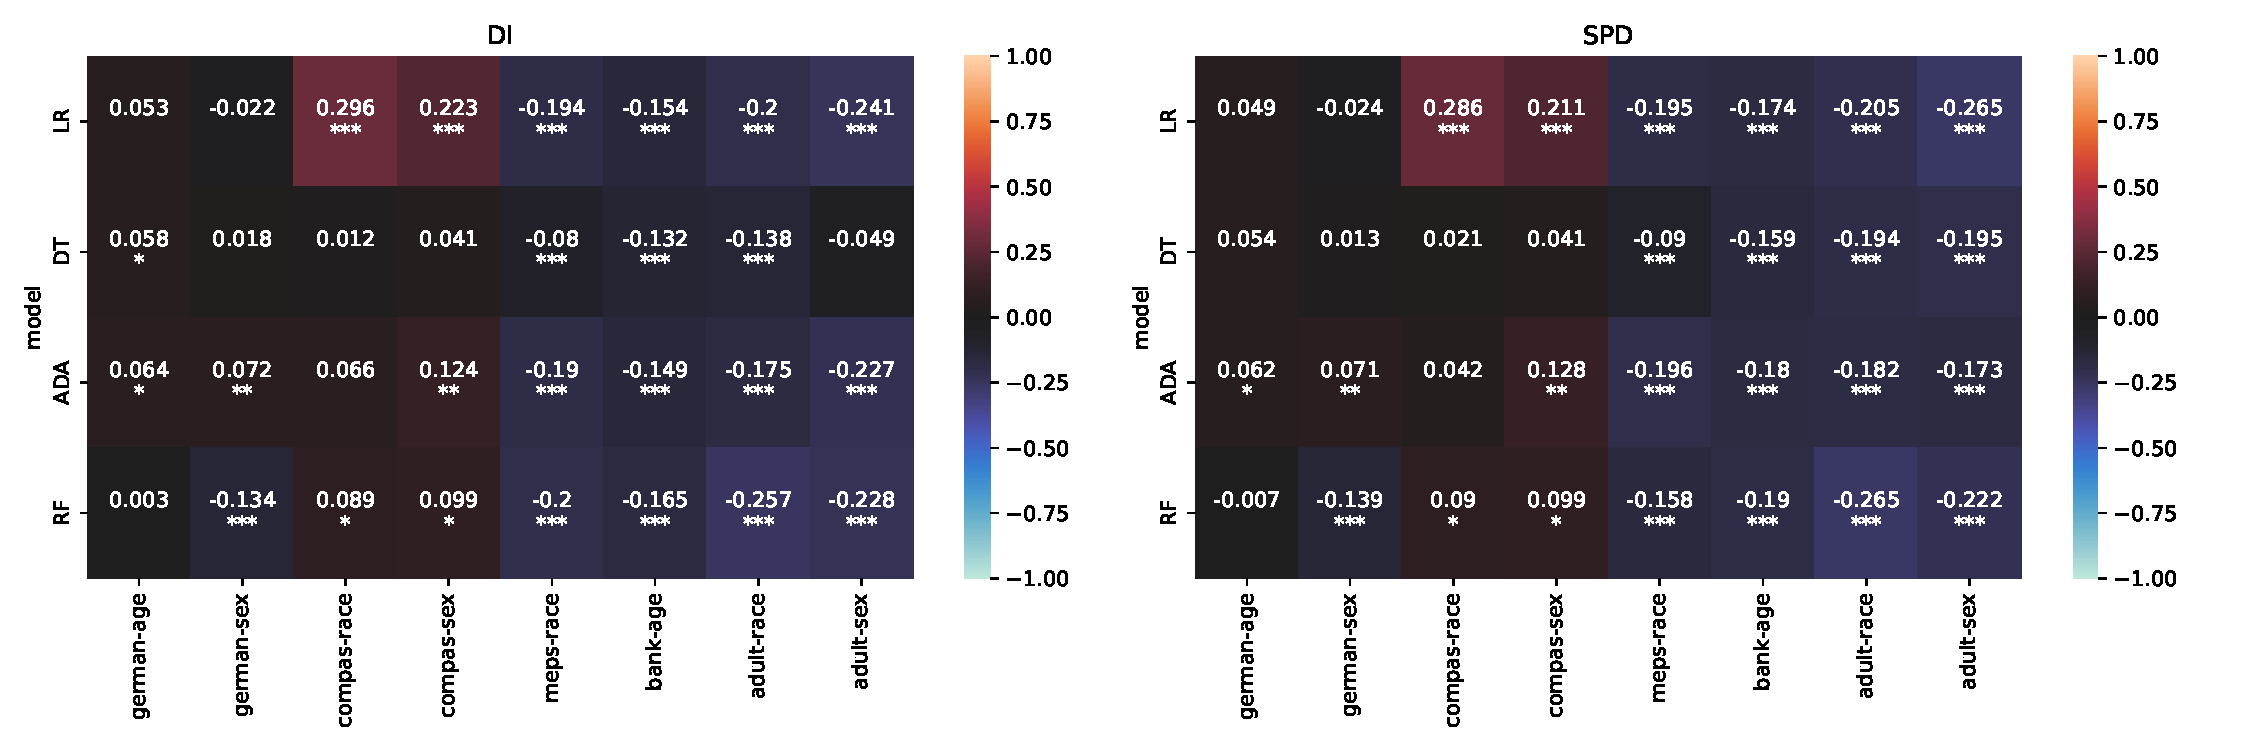
\includegraphics[width=0.95\linewidth]{heatmap--corr--num-features.pdf}
  \caption{Correlation between DFM and MFM across various feature
    sample sizes}
  \label{fig:heatmap--corr--num-features}
\end{figure}

In this section we analyse the relationship between the DFM and MFM
across varying feature sample sizes in the training dataset. In
contract to Section \ref{sec:results-training-sets}, we change the
number of features in the training set and randomise the feature order
in each iteration. Figure \ref{fig:heatmap--corr--num-features}
presents the correlation between the DFM and MFM across all feature
sample sizes. We primarily notice darker colors indicating that there
is no significant correlation between the DFM and MFM as the number of
features in the training dataset changes.
Figure \ref{fig:lineplot--num-features--di-spd--bank-age} shows the
relationship between the fairness metrics with the feature sample
sizes in the XXX dataset. We observe that the MFM decreases as the
number of features in the training set is increased while the DFM
remains constant across all feature sample sizes. Our results from the
MFM align with the results reported by Zhang et
al \cite{zhang2021ignorance}. From Equation \ref{eq:di-data}
and \ref{eq:spd-data}, the DFM remains constant across all feature set
samples since the underlying distribution of the data in the training
set does not change. This explains the lack of significant correlation
between the DFM and MFM. The larger datasets show a more negative
correlation. This could however be due to the change in training set
distribution due to the training-testing split as explained
in \ref{sec:results-full-data} and \ref{sec:results-smaller-data}.

\begin{figure}
  \centering
  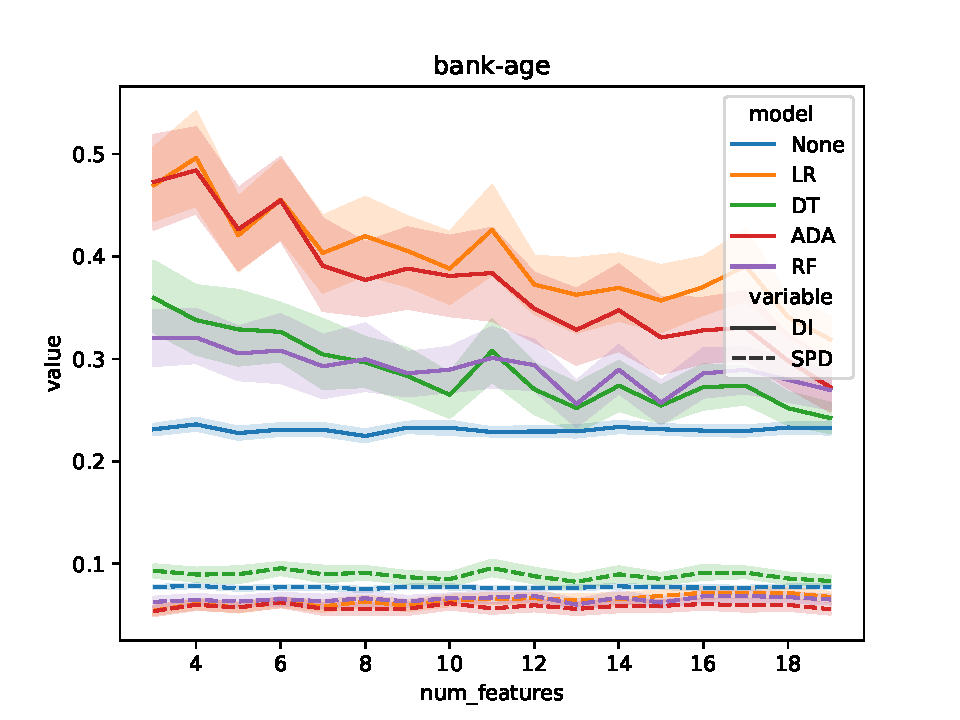
\includegraphics[width=0.95\linewidth]{lineplot--num-features--di-spd--bank-age.pdf}
  \caption{Relationship between fairness metrics and feature sample
    sizes in bank-age dataset}
  \label{fig:lineplot--num-features--di-spd--bank-age}
\end{figure}

\section{Discussion}\label{sec:discuss}

The presence of a positive correlation (and a linear relationship)
between the DFM and MFM indicates that the DFM provides an accurate
depiction of the fairness issues in the model. In such cases, we can
consider only testing the data thus minimising testing efforts. The
presence of a negative correlation indicates that the model was able
to learn from the training set and make fairer decisions. The presence
of no correlation indicates no relationship between the DFM and MFM.
In both cases, no minimisation can be made as both data and model need
to be tested.

%% Arie: fairness should not be related to size of data but we find
%% out that it is; is this a limitation of the type of fairness
%% (group) that we are working with?

%% summarise the overall findings of the study; we cannot always rely
%% only testing the data; leads to limitations of current fairness
%% metrics used in the industry (it does not take the engineering
%% process into account!); however in cases where we can rely on data
%% testing; it has several benefits...

%% mention the early detection angle (this is the over arching theme
%% of my phd so far)

%% mention the test prioritisation/minimisation angle which links into
%% sustainability

%% we can also (briefly) touch upon the explainability angle using the
%% example of decision trees?

%% there is a limitation in the current DFM; they do not account for
%% features in the dataset; another conclusion is that we cannot rely
%% on DFM when experimenting with feature sets; we have to test both
%% data and model.

\section{Threats to Validity}\label{sec:threats}

%% significance of correlation is not reliable for sample size less
%% than 500 (limitation of scipy's implementation of spearman
%% correlation algorithm); mention that we validated correlation with
%% linear regression; we also explored non-linear relationships: if we
%% find non linear relationship then we can say that the models
%% introduce the non-linearity, if not we still have a good addition;

%% we are picking a subset of the dataset that strikes a good balance
%% between performance while capturing various fairness issues; thus
%% each sub-subset can be considered a real-world dataset. threat: we
%% are grossly generalising this threshold, it depends on the dataset;
%% consider making this dynamic

%% TODO we did not look at the underlying distribution of the training
%% dataset (which is biased to begin with); it will be interesting to
%% evaluate if we can minimize fairness testing when we utilise bias
%% mitigation techniques

% note on linear regression model: we used ordinary-least squares with
% degree 1 to estimate the fit; we tried different degrees with
% model=DT and dataset=adult-sex; we also investigated baysian linear
% regression

% pvalue for scipy.stats.spearmanr is not reliable for datasets less
% than 500 examples; this is a threat for the full-data experiment
% since we only have 50 observations per model-dataset combo; this
% means that with more iterations we may see a correlation with
% significance where currently there is none; but this does not change
% our final recommendation which is to test with both data & model in
% these cases

\section{Conclusion}\label{sec:conclude}
%% TODO

\bibliographystyle{named}
\bibliography{report}

\end{document}

